\Variant{05.10.2025 (2-smena)}
\QQ{1}{$x$ va $y$ ning ixtiyoriy natural qiymatlarida qaysi ifoda juft son böladi?
\Opts{$x^2+y^2$}{$xy+y$}{$(x+y)\cdot x$}{$(x+y)\cdot x\cdot y$}}
\QQ{2}{Hisoblang:
\[3{,}0(45)-1{,}(08)+2{,}0(45)\]
\Opts{$4{,}(08)$}{$4{,}(05)$}{$4{,}(02)$}{$4{,}(01)$}}
\QQ{3}{Kinoteatrda har bir qatordagi örindiqlar soni qatorlardan $4$ ga köp. Jami örindiqlar soni $60$ ta. (Har bir qatordagi örindiqlar soni teng). Neçta qator bor?
\Opts{$10$}{$4$}{$6$}{$8$}}
\QQ{4}{$3$ metr adras va $5$ metr atlas narxi $215\,000$ söm. Adras $12\%$, atlas $8\%$ arzonlaşganda narxi $194\,200$ söm böldi. Dastlab adrasning narxi atlas narxidan qança qimmat edi?
\Opts{$5500$}{$5000$}{$6000$}{$6500$}}
\QQ{5}{Hisoblang:
\[\frac{36^3+73^3}{37^3+73^3}\]
\Opts{$\dfrac{105}{110}$}{$\dfrac{107}{108}$}{$\dfrac{109}{110}$}{$\dfrac{110}{111}$}}
\QQ{6}{Hisoblang:
\[\sqrt{12+2\sqrt{19{,}25-\sqrt{19+6\sqrt2}}}\]
\Opts{$2+\sqrt2$}{$2-\sqrt2$}{$3+\sqrt2$}{$3-\sqrt2$}}
\QQ{7}{$a=\sqrt[6]{26}$, $b=\sqrt[3]5$, $c=\sqrt3$ sonlarni kamayiş tartibida yozing.
\Opts{$c>b>a$}{$a>b>c$}{$c>a>b$}{$a>c>b$}}
\QQ{8}{Arifmetik progressiyada $\begin{cases}a_9=3a_3\\ a_8=2(a_3+4)\end{cases}$ berilgan bölsa, $S_{10}$ ni toping.
\Opts{$110$}{$120$}{$220$}{$210$}}
\QQ{9}{Ösuvçi arifmetik progressiyani taşkil qiluvçi $a$, $b$, $c$ sonlar yiğindisi $12$ ga teng. $a+1$; $b$; $c+1$ geometrik progressiyani taşkil qilsa, arifmetik progressiya ayirmasi va geometrik progressiya maxraji yiğindisini toping.
\Opts{$3$}{$4$}{$5$}{$6$}}
\QQ{10}{Agar $\left(\dfrac1{125}\right)^{a^2+4ab}=\left(\sqrt[3]{625}\right)^{3a^2-10ab}$ tenglik örinli bölsa ($a\ne0$), $\dfrac ab$ ni toping.
\Opts{$\dfrac2{21}$}{$\dfrac4{21}$}{$\dfrac5{21}$}{$-\dfrac4{21}$}}
\QQ{11}{Agar $(a+b-5)^2+(b-2c+3)^2+(3c+a-10)^2=0$ bölsa, $a^3+b^3+c^3$ ning qiymatini toping.
\Opts{$57$}{$73$}{$58$}{$65$}}
\QQ{12}{$\dfrac{|\sin x|}{\sin x}=x$ tenglama neçta haqiqiy yeçimga ega?
\Opts{$1$}{$2$}{Haqiqiy yeçimga ega emas}{Çeksiz köp yeçimga ega}}
\QQ{13}{Tenglamaning eng kiçik musbat ildizini toping.
\[\cos^22x+\cos^23x+\cos^210x+\cos^211x=2\]
\Opts{$\dfrac\pi{14}$}{$\dfrac\pi{26}$}{$\dfrac\pi{16}$}{$\dfrac\pi{13}$}}
\QQ{14}{$2025^x+2026\cdot2025^{1-x}=4051$ tenglamaning haqiqiy ildizlari neçta?
\Opts{$1$}{$2$}{$3$}{yeçimga ega emas}}
\QQ{15}{Tenglama neçta haqiqiy ildizga ega?
\[\log_{3x+4}\left(4x^2+12x+9\right)+\log_{2x+3}\left(6x^2+17x+12\right)=4\]
\Opts{$1$}{$2$}{$3$}{yeçimga ega emas}}
\QQ{16}{$x^3-\left(3+\sqrt3\right)x+3=0$ tenglama neçta haqiqiy ildizga ega?
\Opts{$1$}{$2$}{$3$}{yeçimga ega emas}}
\QQ{17}{$\left(x^2+1\right)^{(x-2)(x+2)}\ge\left(x^2+1\right)^{12}$ tengsizlikning $x$ qabul qilmaydigan neçta butun sonlar bor?
\Opts{$8$}{$7$}{$6$}{$5$}}
\QQ{18}{Tengsizlikni yeçing:
\[\frac{x^3-1}{2x^2-3x+1}>1\]
\Opts{$\left(0;\,\dfrac12\right)\cup(1;\,\infty)$}{$\left(\dfrac12;\,1\right)\cup(1;\,\infty)$}{$\left(\dfrac14;\,\dfrac12\right)\cup(1;\,\infty)$}{$\left(\dfrac14;\,1\right)\cup(1;\,\infty)$}}
\QQ{19}{$\dfrac6{\sqrt x+1}>2$ tengsizlikning butun yeçimlari yiğindisini toping.
\Opts{$4$}{$6$}{$5$}{$3$}}
\QQ{20}{Agar $f(x)=(2+x)\left(2x+\dfrac1x\right)$ bölsa, $\dfrac{f\left(\frac12\right)}{f(2)}$ ni toping.
\Opts{$\dfrac5{12}$}{$\dfrac7{12}$}{$\dfrac{11}{12}$}{$\dfrac{15}{12}$}}
\QQ{21}{Aniq integralni hisoblang:
\[\int_0^{\frac\pi2}\frac{dx}{12\cos x-5\sin x+13}\]
\Opts{$\dfrac15$}{$\dfrac12$}{$\dfrac1{10}$}{$1$}}
\QQ{22}{$f(x)=x^3-x^2-7x+6$ funksiya grafigiga $x_0=2$ nuqtada ötkazilgan urinma $Ox$ öqi bilan hosil qilgan ötkir burçakni toping.
\Opts{$30^\circ$}{$45^\circ$}{$60^\circ$}{$75^\circ$}}
\QQ{23}{$ABC$ uçburçakka markazi $O$ nuqtada bölgan aylana içki çizilgan. $AO$ töğri çiziq $BC$ tomonni $D$ nuqtada kesadi. Agar $AB=DC$, $BD=4$ va $AC=9$ ga teng bölsa, $AD$ kesma uzunligini toping.
\qfig{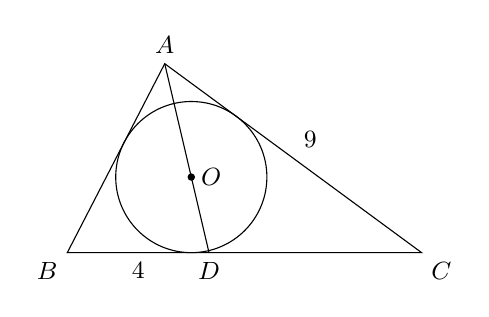
\begin{tikzpicture}[scale=0.45,font=\small]
\coordinate (B) at (0,0); \coordinate (C) at (10,0); \coordinate (A) at (2.75,5.333); \coordinate (D) at (4,0); \coordinate (O) at (3.5,2.133);
\draw (A)--(B)--(C)--cycle; \draw (A)--(D); \draw (O) circle (2.133); \fill (O) circle (3pt);
\node[above] at (A) {$A$}; \node[below left] at (B) {$B$}; \node[below right] at (C) {$C$}; \node[below] at (D) {$D$}; \node[right] at (O) {$O$};
\node[below] at (2,0) {$4$}; \node[above right] at (6.4,2.7) {$9$};
\end{tikzpicture}}
\Opts{$\sqrt{29}$}{$\sqrt{30}$}{$\sqrt{31}$}{$\sqrt{26}$}}
\QQ{24}{$\dfrac{\cos^2x+6\cos x+9}{\sin^2x}$ ifoda $\left[\dfrac\pi3;\,\dfrac{2\pi}3\right]$ oraliqdagi eng kiçik qiymatini toping.
\Opts{$5$}{$9$}{$8$}{$10$}}
\QQ{25}{Rasmdagi maʼlumotlar asosida böyalgan soha yuzini toping ($O$ — aylana markazi).
\qfig{\begin{tikzpicture}[scale=1.1,font=\small]
\coordinate (O) at (0,0); \coordinate (P1) at (100:2); \coordinate (P2) at (160:2); \coordinate (P3) at (220:2); \coordinate (P4) at (340:2);
\fill[qfill] (P3)--(O)--(P1)--(P4)--cycle;
\draw (O) circle (2); \draw (P1)--(P2)--(P3)--(P4)--(P1); \draw (P3)--(O)--(P1); \fill (O) circle (1.3pt); \node[above right] at (O) {$O$};
\draw ($(P3)!0.35cm!(P2)$) arc (100:40:0.35cm); \node at ($(P3)+(70:0.62)$) {\scriptsize$60^\circ$};
\node[above left] at ($(P1)!0.5!(P2)$) {$2$}; \node[left] at ($(P2)!0.5!(P3)$) {$2$}; \node[below] at ($(P3)!0.5!(P4)$) {$2\sqrt3$};
\end{tikzpicture}}
\Opts{$\sqrt3$}{$2\sqrt3$}{$3\sqrt3$}{$4\sqrt3$}}
\QQ{26}{Uçburçakning tomonlari $AB=5$, $BC=4$ va $AC=3$ ga teng. $C$ uçidan $AB$ tomonga $CD$ bissektrisa va $CM$ mediana tuşirilgan. $M$ va $D$ nuqtalar orasidagi masofani toping.
\Opts{$\dfrac57$}{$\dfrac5{14}$}{$\dfrac7{10}$}{$\dfrac9{35}$}}
\QQ{27}{$ABCD$ teng yonli trapetsiyaning ($BC\parallel AD$) diagonallari $O$ nuqtada perpendikulyar kesişadi. $KL$ — örta çiziq, u $AC$ va $BD$ diagonallarni mos ravişda $M$ va $N$ nuqtalarda kesadi. Agar $MN=4$, $CD=4\sqrt{15}$ bölsa, böyalgan soha yuzini toping.
\qfig{\begin{tikzpicture}[scale=0.3,font=\small]
\coordinate (A) at (0,0); \coordinate (D) at (18.97,0); \coordinate (B) at (4,14.97); \coordinate (C) at (14.97,14.97); \coordinate (O) at (9.483,9.487);
\coordinate (K) at (2,7.483); \coordinate (L) at (16.97,7.483); \coordinate (M) at (7.483,7.483); \coordinate (N) at (11.48,7.483);
\fill[qfill] (K)--(O)--(A)--cycle;
\draw (A)--(B)--(C)--(D)--cycle; \draw (A)--(C); \draw (B)--(D); \draw (K)--(L); \draw (K)--(O);
\draw ($(O)!0.5cm!(C)$) -- ($($(O)!0.5cm!(C)$)!1!-90:(O)$) -- ($(O)!0.5cm!(B)$);
\node[below left] at (A) {$A$}; \node[above left] at (B) {$B$}; \node[above right] at (C) {$C$}; \node[below right] at (D) {$D$};
\node[left] at (K) {$K$}; \node[right] at (L) {$L$}; \node[below] at (M) {$M$}; \node[below] at (N) {$N$}; \node[right] at (9.9,9.5) {$O$};
\node[below] at (9.48,7.483) {$4$}; \node[right] at (16.6,11.6) {$4\sqrt{15}$};
\end{tikzpicture}}
\Opts{$26$}{$4$}{$3$}{$6$}}
\QQ{28}{$ABCDE$ muntazam beşburçakning barça diagonallari kesişişidan $FGHKL$ muntazam beşburçak hosil qilindi. Agar $FG=2$ ga teng bölsa, $ABCDE$ muntazam beşburçak perimetrini toping.
\qfig{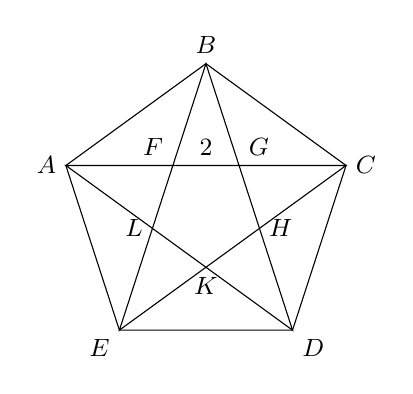
\begin{tikzpicture}[scale=0.42,font=\small]
\coordinate (B) at (0.000,4.454); \coordinate (C) at (4.236,1.376); \coordinate (D) at (2.618,-3.603); \coordinate (E) at (-2.618,-3.603); \coordinate (A) at (-4.236,1.376);
\coordinate (F) at (-1.000,1.376); \coordinate (G) at (1.000,1.376); \coordinate (H) at (1.618,-0.526); \coordinate (K) at (0.000,-1.701); \coordinate (L) at (-1.618,-0.526);
\draw (A)--(B)--(C)--(D)--(E)--cycle; \draw (A)--(C)--(E)--(B)--(D)--cycle;
\node[above] at (B) {$B$}; \node[right] at (C) {$C$}; \node[below right] at (D) {$D$}; \node[below left] at (E) {$E$}; \node[left] at (A) {$A$};
\node[above left] at (F) {$F$}; \node[above right] at (G) {$G$}; \node[right] at (H) {$H$}; \node[below] at (K) {$K$}; \node[left] at (L) {$L$}; \node[above] at (0,1.376) {$2$};
\end{tikzpicture}}
\Opts{$20$}{$5\left(3-\sqrt5\right)$}{$5\left(3+\sqrt5\right)$}{$25$}}
\QQ{29}{Rasmda muntazam oltiburçak tasvirlangan. $E$ nuqtaning koordinatalar köpaytmasini toping.
\qfig{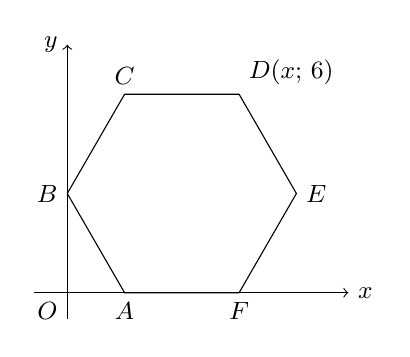
\begin{tikzpicture}[scale=0.42,font=\small]
\draw[->] (-1,0)--(8.5,0) node[right] {$x$}; \draw[->] (0,-0.8)--(0,7.5) node[left] {$y$};
\draw (0,3)--(1.732,6)--(5.196,6)--(6.928,3)--(5.196,0)--(1.732,0)--cycle;
\node[left] at (0,3) {$B$}; \node[above] at (1.732,6) {$C$}; \node[above right] at (5.196,6) {$D(x;\,6)$}; \node[right] at (6.928,3) {$E$}; \node[below] at (5.196,0) {$F$}; \node[below] at (1.732,0) {$A$}; \node[below left] at (0,0) {$O$};
\end{tikzpicture}}
\Opts{$8$}{$9$}{$9\sqrt3$}{$12\sqrt3$}}
\QQ{30}{$ABC$ töğri burçakli uçburçak tekisligiga $C$ uçiga $CD$ perpendikulyar ötkazilgan. Katetlari $AC=15$, $BC=20$ va $CD=35$ ga teng bölsa, $D$ nuqtadan $AB$ tomongaça bölgan eng qisqa masofani toping.
\Opts{$36$}{$37$}{$40$}{$39$}}
\QQ{31}{Rasmdagi maʼlumotlar asosida $(A\cup B)'\cup C$ töplamning elementlar sonini toping.
\qfig{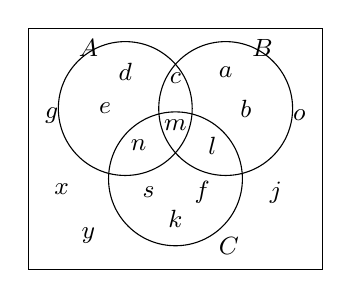
\begin{tikzpicture}[scale=0.85,font=\small]
\draw (-2.2,-2.1) rectangle (2.2,1.5);
\draw (-0.75,0.3) circle (1); \draw (0.75,0.3) circle (1); \draw (0,-0.75) circle (1);
\node at (-1.3,1.2) {$A$}; \node at (1.3,1.2) {$B$}; \node at (0.8,-1.75) {$C$};
\node at (-0.75,0.85) {$d$}; \node at (-1.05,0.3) {$e$}; \node at (0,0.75) {$c$}; \node at (0.75,0.85) {$a$}; \node at (1.05,0.3) {$b$};
\node at (0,0.05) {$m$}; \node at (-0.55,-0.25) {$n$}; \node at (0.55,-0.25) {$l$};
\node at (-0.4,-0.95) {$s$}; \node at (0.4,-0.95) {$f$}; \node at (0,-1.35) {$k$};
\node at (-1.85,0.2) {$g$}; \node at (1.85,0.2) {$o$}; \node at (-1.7,-0.9) {$x$}; \node at (-1.3,-1.6) {$y$}; \node at (1.5,-0.95) {$j$};
\end{tikzpicture}}
\Opts{$8$}{$9$}{$10$}{$11$}}
\QQ{32}{$(x+2y)^5$ yoyilmasining koeffitsiyentlar yiğindisini toping.
\Opts{$32$}{$243$}{$432$}{$512$}}
\QQ{33}{\Moslash{Hajmi $32\sqrt3\pi$ ga teng bölgan şarga silindr içki çizilgan.}{A) $16\sqrt2\pi$\par B) $64\pi$\par C) $24\pi$\par D) $8\sqrt2\pi$\par E) $32\sqrt2\pi$\par F) $32\pi$}{Silindr hajmining eng katta qiymatini toping.}{Silindr yon sirtining eng katta qiymatini toping.}{Silindr hajmi eng katta bölsa, yon sirti yuzini toping.}}
\QQ{36}{Tenglamalar sistemasi bitta haqiqiy yeçimga ega bölsa,
\[\begin{cases}\log_3\left(x^4y^2-a\right)=1+\log_3\left(1+ax^2y^2\right)\\[2pt] 2^{\frac1y}=4^{|x|+1}\end{cases}\]
\AB{$a$ larning yiğindisini toping.}{$x+y$ ning qiymatini toping.}}
\QQ{37}{Tenglamani yeçing.
\[\cos^2x\cos2x+\cos4x+\cos3x\cos x+2\cos^4x=\frac1{2\sin\frac x2}\]
\AB{Tenglamaning eng kiçik musbat yeçimini toping.}{$\left(-\dfrac\pi2;\,\dfrac\pi2\right)$ oraliqda neçta yeçimga ega?}}
\QQ{38}{$f(x)$ çiziqli funksiya va $g(x)$ kvadrat funksiya uçun $f(2)=5$, $g(x-1)=x^2+1$ örinli bölsa,
\AB{$g(x)$ ning eng kiçik qiymatini toping.}{$f^{-1}\bigl(g(1)\bigr)$ ni hisoblang.}}
\QQ{39}{$f(x)=e^{ax^2+bx+1}$ funksiyada $f(1)=f(0)=f'(0)$ tenglik örinli bölsa,
\AB{$\dfrac ab$ ning qiymatini toping.}{$[-1{,}5;\,2]$ oraliqda $f(x)$ funksiyaning eng katta qiymati $m$ bölsa, $\ln m$ ning qiymatini toping.}}
\QQ{40}{$f(x)=ax^2+bx+c$ parabolaning simmetriya öqi $x=4$, u koordinata boşidan ötadi. $g(x)=-|x+m|+n$ funksiya grafigi koordinata boşidan va parabolaning uçidan ötadi hamda parabola bilan $(6;\,3)$ nuqtada ham kesişadi.
\qfig{\begin{tikzpicture}[scale=0.5,font=\small]
\fill[qfill] (0,0)--(4,4) -- plot[domain=4:6,samples=30] (\x,{-\x*\x/4+2*\x}) -- cycle;
\draw[->] (-1.2,0)--(10.5,0) node[right] {$x$}; \draw[->] (0,-2.2)--(0,6.2) node[left] {$y$};
\draw[thick,domain=-0.4:8.6,samples=100] plot (\x,{-\x*\x/4+2*\x});
\draw[thick] (-1.2,-1.2)--(4.5,4.5)--(10,-1);
\draw (0,0)--(6,3); \draw[dashed] (4,0)--(4,4);
\fill (4,4) circle (2.5pt); \fill (6,3) circle (2.5pt); \fill (8,0) circle (2.5pt);
\node[below] at (8,0) {$(8;\,0)$}; \node[right] at (6.1,3.2) {$(6;\,3)$}; \node[below] at (4,0) {$4$}; \node[below left] at (0,0) {$O$};
\node[right] at (5.3,5.3) {$f(x)=ax^2+bx+c$}; \node[right] at (9,-1.5) {$g(x)=-|x+m|+n$};
\end{tikzpicture}}
\AB{$n-m$ ning qiymatini toping.}{Böyalgan soha yuzini toping.}}
\QQ{41}{$ABC$ töğri burçakli uçburçak ($\angle A=90^\circ$) içida radiusi $5$ cm bölgan ikkita bir xil aylana özaro urinadi. Ikkala aylana $BC$ gipotenuzaga, biri $AB$ ga, ikkinçisi $AC$ ga urinadi. Aylanalar markazlaridan ötuvçi töğri çiziq $AB$ va $AC$ ni $E$ va $D$ nuqtalarda kesadi. $BC=35$ cm bölsa,
\qfig{\begin{tikzpicture}[scale=0.17,font=\small]
\coordinate (B) at (0,0); \coordinate (C) at (35,0); \coordinate (A) at (12.6,16.8); \coordinate (E) at (3.75,5); \coordinate (D) at (28.33,5);
\draw (A)--(B)--(C)--cycle; \draw (E)--(D); \draw (10,5) circle (5); \draw (20,5) circle (5);
\draw ($(A)!0.9cm!(B)$) -- ($($(A)!0.9cm!(B)$)!1!90:(A)$) -- ($(A)!0.9cm!(C)$);
\draw (20,5)--(22.94,9.0); \node[above] at (19.7,5.3) {\scriptsize$5$}; \node[above] at (10,5) {\scriptsize$5$};
\node[above] at (A) {$A$}; \node[below left] at (B) {$B$}; \node[below right] at (C) {$C$}; \node[left] at (E) {$E$}; \node[right] at (D) {$D$}; \node[below] at (17.5,0) {$35$};
\end{tikzpicture}}
\AB{$ADE$ uçburçak yuzini toping.}{$ABC$ uçburçak yuzini toping.}}
\QQ{42}{Rasmda uçlari $A\left(2;\,2\sqrt3\right)$, $B\left(5;\,5\sqrt3\right)$, $C\left(9;\,3\sqrt3\right)$ va $D\left(3;\,\sqrt3\right)$ bölgan törtburçak tasvirlangan. Agar $\angle BAD=\beta$ bölsa,
\qfig{\begin{tikzpicture}[scale=0.45,font=\small]
\draw[->] (-1,0)--(11,0) node[right] {$x$}; \draw[->] (0,-0.8)--(0,10) node[left] {$y$};
\fill[qfill] (2,3.464)--(5,8.660)--(9,5.196)--(3,1.732)--cycle;
\draw (2,3.464)--(5,8.660)--(9,5.196)--(3,1.732)--cycle;
\foreach \p in {(2,3.464),(5,8.660),(9,5.196),(3,1.732)} \fill \p circle (3pt);
\node[left] at (2,3.464) {$A\left(2;\,2\sqrt3\right)$}; \node[above] at (5,8.660) {$B\left(5;\,5\sqrt3\right)$}; \node[right] at (9,5.196) {$C\left(9;\,3\sqrt3\right)$}; \node[below] at (3,1.732) {$D\left(3;\,\sqrt3\right)$};
\draw ($(2,3.464)!0.6cm!(5,8.660)$) arc (60:-60:0.6cm); \node at (3.25,3.464) {$\beta$};
\end{tikzpicture}}
\AB{$\sin\beta$ ni toping.}{$ABCD$ törtburçak yuzini toping.}}
\QQ{43}{$ABCDE$ beşburçakda $AB$, $BC$, $CD$ va $DE$ tomon örtalarida mos ravişda $M$, $K$, $N$ va $L$ nuqtalar olingan. $MN$ kesma örtasidan $P$, $KL$ kesma örtasidan $T$ nuqta olindi. Agar $AP=AE=12$ va $\angle PAE=60^\circ$ ga teng bölsa,
\qfig{\begin{tikzpicture}[scale=0.24,font=\small]
\coordinate (A) at (0,0); \coordinate (B) at (8,8); \coordinate (C) at (20,4); \coordinate (D) at (20,-12); \coordinate (E) at (6,-10.392);
\coordinate (M) at (4,4); \coordinate (K) at (14,6); \coordinate (N) at (20,-4); \coordinate (L) at (13,-11.196); \coordinate (P) at (12,0); \coordinate (T) at (13.5,-2.598);
\draw (A)--(B)--(C)--(D)--(E)--cycle; \draw (M)--(N); \draw (K)--(L); \draw (A)--(P)--(T)--(E);
\draw ($(A)!0.9cm!(P)$) arc (0:-60:0.9cm); \node at ($(A)+(-30:1.9)$) {\scriptsize$60^\circ$};
\node[left] at (A) {$A$}; \node[above] at (B) {$B$}; \node[right] at (C) {$C$}; \node[below right] at (D) {$D$}; \node[below] at (E) {$E$};
\node[above left] at (M) {$M$}; \node[above] at (K) {$K$}; \node[right] at (N) {$N$}; \node[below] at (L) {$L$}; \node[above left] at (P) {$P$}; \node[right] at (T) {$T$};
\node[left] at (3,-5.4) {$12$};
\end{tikzpicture}}
\AB{$PT$ kesma uzunligini toping.}{$APTE$ törtburçak yuzini toping.}}
\QQ{44}{Asosi radiusi $3$ ga teng bölgan silindr şaklidagi ğöladan konus va yarim şar öyib olindi. Konusning asosi silindrning bir asosi, yarim şarning asosi silindrning ikkinçi asosi bilan ustma-ust tuşadi, konus uçi esa yarim şar sirtidagi nuqtada. Agar konus yasovçisi $5$ ga teng bölsa,
\qfig{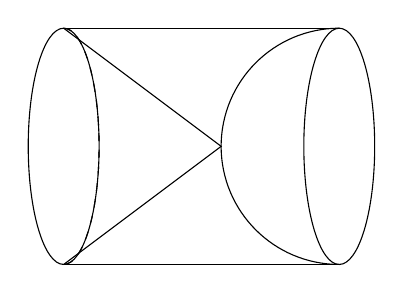
\begin{tikzpicture}[scale=0.5,font=\small]
\draw (0,0) ellipse (0.9 and 3); \draw (7,0) ellipse (0.9 and 3);
\draw (0,3)--(7,3); \draw (0,-3)--(7,-3);
\draw (0,3)--(4,0)--(0,-3); \draw (7,3) arc (90:270:3);
\draw[dashed] (0,3) arc (90:-90:0.9 and 3);
\end{tikzpicture}}
\AB{Öyib olgandan keyingi qolgan jism töla sirtini toping.}{Dastlabki ğöla hajmini toping.}}
\QQ{45}{Quruqlikdagi $A$ nuqtadan $150$ m dagi $T$ nuqtada odam suvda çökyapti. $A$ nuqtadan $B$ nuqtagaça masofa $200$ m. $T$ nuqtada çökyotgan odamga $B$ nuqtadan Anvar yordamga bormoqçi. U birinçi $BC$ böylab $150$ m/daqiqa tezlikda yurdi va $CT$ böyiça $75$ m/daqiqa tezlik bilan suvda suzdi.
\qfig{\begin{tikzpicture}[scale=0.018,font=\small]
\coordinate (A) at (0,0); \coordinate (B) at (200,0); \coordinate (C) at (86.6,0); \coordinate (T) at (0,-150);
\draw (A)--(B); \draw (A)--(T)--(C);
\draw (0,-10)--(10,-10)--(10,0);
\foreach \p in {(A),(B),(C),(T)} \fill \p circle (110pt);
\node[above] at (A) {$A$}; \node[above] at (B) {$B$}; \node[above] at (C) {$C$}; \node[left] at (T) {$T$};
\end{tikzpicture}}
\AB{Anvar yordamga yetib borişi uçun eng kamida qança vaqt ketadi? Javobni butun songaça yaxlitlang.}{Eng kam vaqt sarflanganda Anvar bosib ötgan yöl uzunligini toping ($\sqrt3\approx1{,}7$ deb oling).}}
\Javoblar{D D C B C C C C C D B B B B A C C B B A C B B C B B A C D B D B F C A}{%
\OK{36}{$-3$}{$\dfrac12$}\OK{37}{$\dfrac\pi{11}$}{$5$}\OK{38}{$1$}{$2$}\OK{39}{$-1$}{$\dfrac54$}\OK{40}{$9$}{$\dfrac{19}3$}%
\OK{41}{$\dfrac{3481}{24}$}{$294$}\OK{42}{$\dfrac{\sqrt3}2$}{$13\sqrt3$}\OK{43}{$3$}{$45\sqrt3$}\OK{44}{$75\pi$}{$63\pi$}\OK{45}{$3$ daqiqa}{$285$ m}}
